\section{Refinement-based game semantics}

This section introduces the category $\mathcal{G}$ of games and strategies
we use to interpret the behavior of low-level interacting components.
$\mathcal{G}$ has no high-order structure,
which simplifies the definition of games considerably.
On the other hand,
our definition of strategy is generalized to accomodate specifications,
and the morphisms of $\mathcal{G}$ are equipped with a notion of refinement
suitable for our purposes.

\subsection{Games}

\subsubsection{Elementary games}

The elementary games which underlie
our category of games and strategies
can be decribed in the following way.

\begin{definition}
An \emph{elementary game} is a pair
$A = \langle M_A^\kw{Q}, M_A^\kw{A} \rangle$, where
$M_A^\kw{Q}$ is a set of \emph{questions}, and
$M_A^\kw{A}$ is a set of \emph{answers}.
\end{definition}

The game proceeds as follows:
$\kw{O}$ chooses a question, then
$\kw{P}$ chooses an answer.
Elementary games place no restrictions
on the valid plays,
but this can be specified relationally.

\begin{definition}
A \emph{refinement convention} between elementary games $A_1$ and $A_2$
is a tuple
$\mathbb{C} = \langle W_\mathbb{C}, \preceq_\mathbb{C}^\kw{Q}, \preceq_\mathbb{C}^\kw{A} \rangle$
consisting in a set $W_\mathbb{C}$ of \emph{worlds},
and two relations
${\preceq}_\mathbb{C}^\kw{Q} : \mathcal{R}_{W_\mathbb{C}}(M_{A_1}^\kw{Q},M_{A_2}^\kw{Q})$ and
${\preceq}_\mathbb{C}^\kw{A} : \mathcal{R}_{W_\mathbb{C}}(M_{A_1}^\kw{A},M_{A_2}^\kw{A})$.
We write $\mathbb{C} : \mathcal{R}(A_1, A_2)$.
\end{definition}

Refinement conventions specify a correspondance
between the questions and answers of their source and target games,
which can be extended to plays and strategies.
The use of worlds ensures that the question and answer
are related in a consistent way.
If the source and target are the same game,
this is can be used to specify a set of valid plays
and augment the game with a notion of refinement.

\begin{definition}
A \emph{game with refinement} $\langle A, \preceq_A \rangle$
is an elementary game
$A = \langle M_A^\kw{Q}, M_A^\kw{A} \rangle$
together with a refinement convention
$\preceq_A = \langle W_{\!A}, \preceq_A^\kw{Q}, \preceq_A^\kw{A} \rangle$
such that $\preceq_A^\kw{Q}$ and $\preceq_A^\kw{R}$
are transitive at all worlds.
\end{definition}

In the context of games with refinement,
the valid plays and strategies will be the ones
that are self-related.
Our focus will be the plays and strategies
for the composite game $A \rightarrow B$
described in \S\ref{sec:arrow}.
Before we formally define them,
we start by addressing
the possibility for $\kw{P}$ to silently diverge
and to refuse any question from $\kw{O}$.

\subsubsection{Divergence}

We model internal actions in the following way.
Whenever $\kw{P}$ is to play,
it may instead ``ask for more time''
and play the special move $\tau$,
in which case $\kw{P}$ will retain control.
There is no limit on the number of internal actions that
$\kw{P}$ may perform before playing a regular move;
we say that a strategy \emph{diverges}
when it plays $\tau$ indefinitely.

Internal actions usually correspond to the hidden interactions
within composite systems, and
divergence is an \emph{emergent} phenomenon:
systems that are well-behaved when taken in isolation
may nontheless exhibit divergence when they interact with one another.
As such,
divergence is one of the major sources of complexity
in compositional semantics.

In our setting,
the occurence of internal actions
is observable,
and our definition of simulation
makes no effort
to identify finite sequences of internal actions
which have different lengths.
Instead,
in \S\ref{sec:bigstep}
we introduce an operator $- \backslash \tau^*$
that can be used to normalize strategies
by eliminating altogether all such finite sequences.

\subsubsection{Refusals}

In our model,
$\kw{P}$ may \emph{refuse} a question:
immediately after $\kw{O}$ plays a question,
$\kw{P}$ can play the special move $\kw{\#}$,
after which the game terminates.
In the context of
\emph{horizontal composition} (\S\ref{sec:hcomp}),
this will allow another component to proceed.

Note that a nondeterministic specification
may allow both answering and refusing a given question,
and that refusal must be distinguished from
the absence of behavior
(which in our setting would refine any specification).

%From there, we describe increasingly complex games,
%up to the composite game $A \rightarrow B$.
%Well-bracketed, alternating strategies for this game
%will serve as the morphisms of $\mathcal{G}$.
%
%\subsubsection{Iteration}
%
%If we allow multiple iterations of the game,
%the plays will be paths from $\kw{O}$ in the following graph:
%\[
%  \begin{tikzpicture}[baseline=(O.base)]
%    \node (O) at (0,0) {\kw{O}};
%    \node (P) at (1,0) {\kw{P}};
%    \path [->] (O) edge[bend left] node[auto] {$m$} (P);
%    \path [->] (P) edge[bend left] node[auto] {$n$} (O);
%  \end{tikzpicture}
%  \qquad
%  \begin{array}{c@{\,}l}
%    m &\in M_A^\kw{Q} \\[1ex]
%    n &\in M_A^\kw{A}
%  \end{array}
%\]
%To formalize the relational aspects of iterated elementary games,
%we can adjust the graph above so that its vertices are taken
%from the set of worlds extended with a starting point $\star$,
%and its edges are labelled by \emph{pairs} of related moves:
%\[
%  \begin{tikzpicture}[baseline=(O.base)]
%    \node (O) at (0,0) {$\star$};
%    \node (P) at (2,0) {$w$};
%    \path [->] (O) edge[bend left] node[auto] {$m_1, m_2$} (P);
%    \path [->] (P) edge[bend left] node[auto] {$n_2, n_2$} (O);
%  \end{tikzpicture}
%  \qquad
%  \begin{array}{c}
%    (m_1, m_2) \in {\preceq}_A^\kw{Q} \\[.5ex]
%    w \in W_{\!A} + \star \\[.5ex]
%    (n_1, n_2) \in {\preceq}_A^\kw{A}
%  \end{array}
%\]
%Two sequences of moves $s_1, s_2$
%are related at a world $w$
%if the graph contains a path $s : \star \leadsto w$
%such that $s_1 = \pi_1^*(s)$ and $s_2 = \pi_2^*(s)$.
%A strategy $\sigma_1$ is simulated by a strategy $\sigma_2$ if
%any move $n_1$ of $\sigma_1$ at the position $s_1$
%matches a corresponding move $n_2$ of $\sigma_2$ at the position $s_2$,
%such that $n_1 \preceq_A^\kw{A} n_2$.

\subsubsection{Arrow games}
\label{sec:arrow}

The arrow game $A \rightarrow B$ consists of
nested iterations of the elementary games $A$ and $B$.
In instances of $A$, the roles of $\kw{P}$ and $\kw{O}$ are exchanged;
instances of $B$ proceed normally.
When a new instance is initiated,
the current game is suspended
until the new instance concludes.

Accounting for internal actions and refusals,
the valid plays of $A \rightarrow B$
are described by the following graph:
\[
  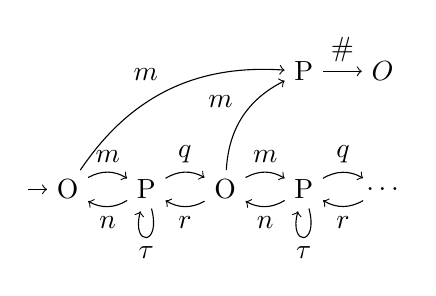
\begin{tikzpicture}[baseline=(O1.base)]
    \node (O1) at (0,0) {\kw{O}};
    \node (P1) at (1,0) {\kw{P}};
    \node (O2) at (2,0) {\kw{O}};
    \node (P2) at (3,0) {\kw{P}};
    \node (O3) at (4,0) {$\ldots$};
    \node (R) at (3,1.5) {\kw{P}};
    \node (H) at (4,1.5) {$\kw{O}$};
    \path [->] (R) edge node[auto] {$\#$} (H);
    \path [->] (-0.5,0) edge (O1);
    \path [->] (O1) edge[bend left] node[auto] {$m$} (P1);
    \path [->] (O1) edge[bend left] node[auto] {$m$} (R);
    \path [->] (P1) edge[bend left] node[auto] {$n$} (O1);
    \path [->] (P1) edge[bend left] node[auto] {$q$} (O2);
    \path [->] (P1) edge[loop below] node[auto] {$\tau$} (P1);
    \path [->] (O2) edge[bend left] node[auto] {$r$} (P1);
    \path [->] (O2) edge[bend left] node[auto] {$m$} (P2);
    \path [->] (O2) edge[bend left] node[auto] {$m$} (R);
    \path [->] (P2) edge[bend left] node[auto] {$n$} (O2);
    \path [->] (P2) edge[bend left] node[auto] {$q$} (O3);
    \path [->] (P2) edge[loop below] node[auto] {$\tau$} (P2);
    \path [->] (O3) edge[bend left] node[auto] {$r$} (P2);
  \end{tikzpicture}
  \quad
  \begin{array}{c@{\,}lc@{\,}l}
    m &\in M_B^\kw{Q} & q &\in M_A^\kw{Q} \\[1ex]
    n &\in M_B^\kw{A} & r &\in M_A^\kw{A}
  \end{array}
\]
The first move is always a question $m$ played by $\kw{O}$ in $B$.
The player $\kw{P}$ can conclude the current instance of $B$
with an answer $n$, or
initiate an instance of $A$
with a question $q$.
Then $\kw{O}$ can initiate a new instance of $B$
with another $m$, or
conclude any current instance of $A$
with an answer $r$.
This process goes on indefinitely.

%A corresponding relational frame can be defined
%on worlds of the form $\vec{w} \in (W_{\!A} + W_B)^*$.
%The starting state $\varepsilon$ corresponds to
%the leftmost $\kw{O}$ position above.
%The transitions are as follows.
%\[
%  \begin{array}{c@{\qquad}c}
%    \text{For $\lvert \vec{w} \rvert$ even:} &
%    \text{For $\lvert \vec{w} \rvert$ odd:} \\[1ex]
%    \AxiomC{$m_1 \ifr{w \Vdash {\preceq}_B^\kw{Q}} m_2$}
%    \UnaryInfC{$\vec{w} \stackrel{m_1, m_2}{\leadsto} w :: \vec{w}$}
%    \DisplayProof
%    &
%    \AxiomC{$q_1 \ifr{w \Vdash {\preceq}_A^\kw{Q}} q_2$}
%    \UnaryInfC{$\vec{w} \stackrel{q_1, q_2}{\leadsto} w :: \vec{w}$}
%    \DisplayProof
%    \\[3.3ex]
%    \AxiomC{$n_1 \ifr{w \Vdash {\preceq}_B^\kw{A}} n_2$}
%    \UnaryInfC{$w :: \vec{w} \stackrel{n_1, n_2}{\leadsto} \vec{w}$}
%    \DisplayProof
%    &
%    \AxiomC{$r_1 \ifr{w \Vdash {\preceq}_A^\kw{A}} r_2$}
%    \UnaryInfC{$w :: \vec{w} \stackrel{r_1, r_2}{\leadsto} \vec{w}$}
%    \DisplayProof
%  \end{array}
%\]
%As before,
%two sequences of moves are related if
%there is a corresponding path in the graph.

To formalize the plays and strategies of $A \rightarrow B$
in a way that accounts for refinement,
we decouple two aspects of this structure:
On one hand,
the following definition of plays
enforces the alternation between $\kw{O}$ and $\kw{P}$
and specifies how the special moves $\tau$ and $\#$ can be used.

\begin{definition}
Given two elementary games $A$ and $B$,
the moves of the arrow game $A \rightarrow B$
are the questions and answers of $A$ and $B$,
categorized as follows:
\begin{align*}
  M_{A \rightarrow B}^\kw{O} &= M_A^\kw{A} + M_B^\kw{Q} &
  M_{A \rightarrow B}^\kw{Q} &= M_A^\kw{Q} + M_B^\kw{Q} \\
  M_{A \rightarrow B}^\kw{P} &= M_A^\kw{Q} + M_B^\kw{A} &
  M_{A \rightarrow B}^\kw{A} &= M_A^\kw{A} + M_B^\kw{A}
\end{align*}
The \emph{plays} are taken in
the prefix closure $P_{A \rightarrow B}$ of the set:
\[
    (M_{A \rightarrow B}^\kw{O} \tau^*
     M_{A \rightarrow B}^\kw{P})^*
    (\varepsilon + M_{A \rightarrow B}^\kw{O} \#) \,.
\]
\end{definition}

On the other hand,
the ``stack discipline'' associating questions
with their eventual answer is captured by
the way we extend refinement conventions to
the plays of $A \rightarrow B$.

\begin{definition}
Given
$\mathbb{C}_A : \mathcal{R}(A_1, A_2)$ and
$\mathbb{C}_B : \mathcal{R}(B_1, B_2)$,
we define the Kripke frame
labelled by pairs of moves:
\[
    \mathcal{F}_{A \rightarrow B} =
      \langle (W_A + W_B)^*, \leadsto \rangle \,,
\]
where $\leadsto$ is the transition system
defined by the rules:
\[
    \AxiomC{$m_1 \ifr{w \Vdash {\preceq}^\kw{Q}} m_2$}
    \UnaryInfC{$\vec{w} \stackrel{m_1, m_2}{\leadsto} w :: \vec{w}$}
    \DisplayProof
    \quad
    \begin{array}{c}
      \vec{w} \stackrel{\#,\#}{\leadsto} \vec{w} \\[0.7ex]
      \vec{w} \stackrel{\tau, \tau}{\leadsto} \vec{w}
    \end{array}
    \quad
    \AxiomC{$m_1 \ifr{w \Vdash {\preceq}^\kw{A}} m_2$}
    \UnaryInfC{$w :: \vec{w} \stackrel{m_1, m_2}{\leadsto} \vec{w}$}
    \DisplayProof
\]
Then two plays are related at $\vec{w}$
when there is a path from $\varepsilon$ to $\vec{w}$
in $\leadsto$ whose labels project onto the plays:
\[
    \AxiomC{$s : \varepsilon \leadsto^* \vec{w}$}
    \UnaryInfC{$\pi_1^*(s)
       \ifr{\vec{w} \Vdash {\preceq}_{A \rightarrow B}}
       \pi_2^*(s)$}
    \DisplayProof
\]
If
$\langle A, \mathbb{C}_A \rangle$ and
$\langle B, \mathbb{C}_B \rangle$
are two games with refinement, then
a \emph{valid play} of $A \rightarrow B$
is a sequence $s \in P_{A \rightarrow B}$
such that $s \ifr{\vec{w} \Vdash {\preceq}_{A \rightarrow B}} s$
for some $\vec{w}$.
\end{definition}

By analogy with the more usual notion of alternating plays,
we call \emph{even}
the empty play and the plays ending in
a move from $M_{A \rightarrow B}^\kw{P} \cup \{\#\}$, and
we call \emph{odd} the plays ending in
a move from $M_{A \rightarrow B}^\kw{O} \cup \{\tau\}$.
We write $P_{A \rightarrow B}^\kw{even}$ and $P_{A \rightarrow B}^\kw{odd}$
for the corresponding subsets of $P_{A \rightarrow B}$.

\subsection{Strategies}

A strategy for $A \rightarrow B$
is essentially a tree
which gathers the possible interactions of
the system being modeled.
We give a traditional representation
as a prefix-closed set of plays,
then formalize a more direct notion of strategies as
\emph{alternating transition systems}.

\subsubsection{Traces}

In the existing literature,
strategies are usually formalized as prefix-closed sets of plays.
This establishes a connection with trace semantics of process calculi.
In our case,
a strategy given in this form is a set:
\[ \sigma \subseteq P_{A \rightarrow B} \,, \]
which satisfies
for all $st \in P_{A \rightarrow B}$
and $m \in M_{A \rightarrow B}^\kw{O}$:
\begin{itemize}
  \item $st \in \sigma \Rightarrow s \in \sigma$;
  \item $s \in \sigma \wedge sm \in P_{A \rightarrow B}
    \Rightarrow sm \in \sigma$.
\end{itemize}
The first condition ensures that $\sigma$ is prefix-closed,
whereas the second condition ensures that
all possible behaviors of $\kw{O}$ are included
at all reachable positions.

\subsubsection{Nondeterministic functions}

To emphasizes an operational understanding of strategies,
we can also view $\sigma$ as a nondeterministic function:
\[ \sigma : P_{A \rightarrow B}^\kw{odd} \rightarrow
        \mathcal{P}(M_{A \rightarrow B}^\kw{P}) \,, \]
such that for all $s, t \in P_{A \rightarrow B}^\kw{odd}$
and $m, n \in M_{A \rightarrow B}^\kw{P}$:
\[ \sigma(s m t) \ni n \: \Rightarrow \: \sigma(s) \ni m \,. \]
This makes clear that the role of a strategy
is to provide possible next moves at all reachable positions
in the game.

\subsubsection{Alternating transition systems}

A more structural approach is to specify
strategies as transition systems
alternating between a set of states $S$ and
a set of continuations $K$.
States correspond to points in the execution
where $\kw{P}$ is expected to move,
whereas continuations expect a move from $\kw{O}$
and specify how the execution should be resumed.

The initial configuration of the system
is specified by a continuation.
For each continuation $k \in K$
and each possible move $m \in M_{A \rightarrow B}^\kw{O}$
we specify a set of possible \emph{resumptions}
among the following:
\[ r \in \kw{res} ::= s \mid \# \]
If the environment's move is accepted,
the execution can proceed in state $s$.
Alternatively,
a continuation may refuse a given input move,
as indicated by the resumption $\#$.

We associate to each state $s$ a set of possible
behaviors among the following:
\[ b \in \kw{beh} ::=
	\tau \cdot s' \mid
	\underline{m} \cdot k \]
The behavior $\tau \cdot s'$
performs an internal action and transitions to state $s'$;
the behavior $\underline{m} \cdot k$
plays the move $m$ and transitions to the continuation $k$.

For simplicity, and without loss of generality,
we will take the set of continuations
to be defined in terms of $S$ as:
\[ K := M \rightarrow \mathcal{P}(\kw{res}) \,. \]

\begin{definition}
Given two elementary games $A, B$ and a set of states $S$,
an \emph{alternating transition system} is a relation:
\[
  \alpha : S \rightarrow \mathcal{P}(\kw{behavior}(M, S)) \,.
\]
The type of alternating transition systems
will be written as $\kw{ats}_{A \rightarrow B}(S)$.
\end{definition}

To establish a connection with other representations of strategies,
we can define corecursively the set of traces generated by an
alternating transition system as:
\begin{itemize}
  \item $\kw{traces}_\alpha(k) =
         \{ \varepsilon, m, mt \mid r \in k(m) \wedge t \in \kw{traces}(r) \}$
  \item $\kw{traces}_\alpha(\#) = \{ \varepsilon, \# \}$
  \item $\kw{traces}_\alpha(s) =
         \{ \varepsilon, t \mid b \in \alpha(s) \wedge t \in \kw{traces}(b) \}$
  \item $\kw{traces}_\alpha(\tau \cdot s') =
         \{ \varepsilon, \tau t \mid t \in \kw{traces}(s')$
  \item $\kw{traces}_\alpha(\underline{m} \cdot k) =
         \{ \varepsilon, m t \mid t \in \kw{traces}(k)$
\end{itemize}

Strategies can be defined in terms of alternating transition systems
by providing an initial continuation and hiding the set of states.

\begin{definition}[Strategy]
For a set of moves $M$,
a strategy $\sigma = (S, \alpha, k_0)$
is a set of states $S$ together with
an alternating transition system $\alpha : \kw{ats}(M, S)$ and
an initial continuation $k_0 : S \rightarrow \mathcal{P}(\kw{resumption}(S))$.
For a strategy $\sigma = (S, \alpha, k_0)$,
we define its set of traces as
$\kw{traces}(\sigma) = \kw{traces}_\alpha (k_0)$.
\end{definition}

[Advantages: alternation structure baked in,
can be handled by the proof assistant's type system.
Facilitates embedding of operational semantics,
and intuitive operational reasoning.]

[Inconvenient: junk and non unique,
but we don't care because we're going to
define simulations and quotient anyway.]

\subsection{Refinement conventions}








Given two strategies $\sigma_1, \sigma_2$,
we want to formulate a notion of refinement
$\sigma_1 \sqsubseteq \sigma_2$.
To make it possible to relate strategies at different
levels of abstraction,
we will need to specify how the moves of $\sigma_1$
relate to those of $\sigma_2$
as the execution proceeds.
since this is a stateful process,
we formalize this \emph{refinement convention}
as a Kripke logical relation between the two games.

\begin{definition}[Refinement convention]
Given two sets of moves $M_1$, $M_2$,
a refinement convention
is a Kripke logical relation $\mathbb{R} = (W, \leadsto, R_M)$
between $M_1$ and $M_2$.
\end{definition}

We obtain our notion of refinement by extending $\mathbb{R}$
in a natural way,
first to state behaviors and continuation resumptions,
then to simulations of transition systems,
and finally to our refinement of strategies.

\subsection{Simulations}

For a refinement convention $\mathbb{R} : \mathcal{R}_W(M_1, M_2)$,
a Kripke logical relation on states $R : \mathcal{R}_W(S_1, S_2)$
can be extended to resumptions as follows:
\[
  \AxiomC{$s_1 \ifr{w \Vdash R} s_2$}
  \UnaryInfC{$\kw{resume}(s_1) \ifr{w \Vdash R_\kw{r}} \kw{resume}(s_2)$}
  \DisplayProof
  \quad
  \AxiomC{\rule{0pt}{\baselineskip}}
  \UnaryInfC{$\kw{refuse} \ifr{w \Vdash R_\kw{r}} \kw{refuse}$}
  \DisplayProof
\]
For simple state behaviors,
refinement is defined as follows:
\[
  \AxiomC{$s_1' \ifr{w \Vdash R} s_2'$}
  \UnaryInfC{$\tau \cdot s_1' \ifr{w \Vdash R_\kw{b}} \tau \cdot s_2'$}
  \DisplayProof
  \quad
  \AxiomC{\rule{0pt}{\baselineskip}}
  \UnaryInfC{$\Delta \ifr{w \Vdash R_\kw{b}} \Delta$}
  \DisplayProof
  \quad
  \AxiomC{\rule{0pt}{\baselineskip}}
  \UnaryInfC{$b \ifr{w \Vdash R_\kw{b}} \lightning$}
  \DisplayProof
\]
Note that the behavior $\lightning$ is defined as a top element
for refinement,
so that a strategy that goes wrong can be refined arbitrarily
but can only implement a specification that
also goes wrong.
By contrast,
explicit divergence $\Delta$
is only related to itself,
and counts as a specific behavior on par with others.

For interacting state behaviors,
the KLR structure is going to come into play.
Two continuations $k_1, k_2$ are related when
for any world transition,
and any two moves which are related in the new world,
every resumption of $k_1$ has a corresponding resumption in $k_2$:
\[
  R_\kw{k} := \Box (\mathbb{R} \rightarrow \mathcal{P}^+(R_\kw{r}))
\]
Two interactions are related
if there exists a world transition that relates the output moves,
and relates the associated continuations:
\[
  \AxiomC{$(m_1, k_1) \ifr{w \Vdash \Diamond (\mathbb{R} \times R_\kw{k})} (m_2, k_2)$}
  \UnaryInfC{$
	{\underline{m_1} \cdot k_1}
	\: \ifr{w \Vdash R_\kw{b}} \:
	{\underline{m_2} \cdot k_2}$}
  \DisplayProof
\]
Based on these definitions for the refinement of
resumptions and state behaviors,
we can define our notion of simulation.

\begin{definition}[Kripke simulation relation]
For two transition systems
$\alpha_1 : \kw{ats}(S_1, M_1)$,
$\alpha_2 : \kw{ats}(S_2, M_2)$ and
a refinement relation
$\mathbb{R} : \mathcal{R}_W(M_1, M_2)$,
we say that
$R : \mathcal{R}_W(S_1, S_2)$
is a Kripke simulation relation between $\alpha_1$ and $\alpha_2$
when:
\[
    \alpha_1 \ifr{\Vdash R \rightarrow \mathcal{P}^+(R_b)} \alpha_2
\]
We will write $\alpha_1 \le_R \alpha_2$.
\end{definition}

Note that for both states and continuations,
nondeterminism is interpreted as \emph{output} nondeterminism,
as prescribed by the use of the relator $\mathcal{P}^+$.
This means that alternating transition system
implicitely accept all possible inputs from the environment,
although some of them may cause the system to immediately go wrong.
Likewise,
the special resumption $\kw{refuse}$
is taken as a positive, output behavior from the system,
rather than a restriction on the environment ---
this will be important to establish the monotonicity
of the composition operator defined in Sec.~\ref{?}.
This approach corresponds to the saturation requirement on strategies
often found in traditional game semantics,
or notions of receptiveness used in CompCert
and in concurrency theory.

Furthermore, we need to distinguish between mere nondeterminism
and \emph{branching}.
This is explored in the following section.

\subsection{Branching and determinism}

Whereas nondeterminism allows a strategy to posess
multiple observable behaviors,
branching occurs when multiple state transitions
are associated with the same immediate observable behavior.
This can create spurious distinctions,
whereby systems that yield the same sets of traces
cannot be identified by simulation,
and as such we consider it undesirable.
The following definition
formalizes the conditions a transition system must satisfy
to be considered free from branching.

\begin{definition}[Nonbranching transition system]
For given sets of moves and states,
a continuation $k : M \rightarrow \mathcal{P}(\kw{resumption}(S))$
is \emph{nonbranching} if the following property holds:
\[ \forall m \,.\, | k(m) | \le 1 \]
A transition system $\alpha : \kw{ats}(M, S)$ is nonbranching
if the following property holds:
\[ \forall s, m, k_1, k_2 \,.\,
     \alpha(s) \supseteq \{ m \cdot k_1, m \cdot k_2 \} \Rightarrow
     k_1 = k_2 \,, \]
and if for all $s, m, k$ such that $\alpha(s) \ni \underline{m} \cdot k$,
the continuation $k$ is nonbranching.
\end{definition}

Determinism is a stronger property,
and ensures that the system has at most one possible behavior
at any point.
We expect the semantics of concrete systems ---
as opposed to specifications ---
to be deterministic in the following sense.

\begin{definition}[Deterministic transition system]
For given sets of moves and states,
a transition system $\alpha : \kw{ats}(M, S)$
is deterministic if for all $s$, $|\alpha(s)| \le 1$,
and if for all $s, m, k$ such that $\alpha(s) \ni \underline{m} \cdot k$,
the continuation $k$ is nonbranching.
\end{definition}

Note that both nonbranching and determinism
only relate to the behavior of the system.
In both cases,
the environment remains free to play any move.
Abramsky notes in \cite{cspgs}
that [it's one of the good things about game semantics].

\subsection{Internal actions and divergence}

The emergence of silent divergence
is one of the major difficulties
associated with modeling interacting systems.
Indeed,
two systems which, taken in isolation,
only exhibit reactive behavior,
can nonetheless become silently divergent when composed together,
if it is possible to interact with each other continuously
without intervening communication with the outside.

An operational description of this phenomenon
models this internal interaction explicitly
in the form of silent actions $\tau$.
When comparing the behavior of two systems,
finite sequences of $\tau$'s will be considered equivalent.
However,
silent divergence in the form of an infinite sequence of $\tau$'s
can only correspond to another infinite sequence.
This is usually addressed by the introduction of
sophisticated notions of simulation,
such as the \emph{measure simulations} used for instance in CompCert.

On the other hand,
in most work on denotational semantics,
including traditional game semantics such as \cite{pcfgs},
[complicated fixpoints] 

Our model includes a notion of internal action $\tau$,
which makes it possible to handle silent divergence explicitely
rather than through sophisticated domain-theoretic constructions.
However,
note that the notion of simulation we have defined
does not allow any variation
in the number of internal transitions
between the two transition systems being related.
Nevertheless,
composition operators remain monotonic
under this definition of simulation,
because [...]
Normalize using the following operator.

\begin{definition}[Observation operator]
For a transition system $\alpha : \kw{ats}(M, S)$,
we define the \emph{observations} transition system
$\mathcal{O}(\alpha)$ as follows.
A behavior $r : \kw{behavior}(M, S)$ is said to be
\emph{observable} if $r \ne \tau \cdot s$ for all $s \in S$.
A state $s' \in S$ is said to be \emph{reachable} from $s \in S$
if there is a sequence $s_0, s_1, \ldots s_n$ such that
$s_0 = s$, $s_n = s'$,
and for all $0 \le i < n$
there is a transition $\alpha(s_i) \ni \tau \cdot s_{i+1}$.
A state $s$ is said to be \emph{silently divergent}
if there is an infinite sequence $s_0, s_1, \ldots$
such that $s_0 = s$ and for all $i$,
there is a transition $\alpha(s_i) \ni \tau \cdot s_{i+1}$.
Then the observations transition system is defined as:
\begin{align*}
    \mathcal{O}(\alpha)(s) = &\{ r \:|\: r \mbox{ is observable } \wedge
         \exists s' \,.\, s \rightarrow^* s' \wedge
		\alpha(s') \ni r \} \\
      \cup &\{ \Delta \:|\: s \mbox{ is silently divergent} \}
\end{align*}
\end{definition}

Properties:
preserve nonbranching (if that's defined in the right way), determinism.
Monotonic.

\subsection{Composite games}




\subsection{Horizontal composition}





